% Moved out of the 8-page paper on Oct 20, 2026 to fit the page limit; for the supplement (due Nov 23).
% Shift point clouds: fig/qual_shift.pdf (code/fig_paper_points.py).

% ---- from sec/3_method.tex ----
\subsection{Amortised verification}
\label{sec:amortise}
Over a stream of queries, a gradient-boosted regressor learns to predict the certificate score from the physical inputs and simple statistics of the generated motion.
Probes are skipped when the prediction, inflated by a split-conformal margin, is below $\tau$.
The margin is calibrated on a random 10\% of queries that are always probed (audits), which keeps the skip rule valid for a stationary stream.
% src: Phase 5a (audit 0.10, delta 0.05)


% ---- from sec/5_results.tex ----
\subsection{Amortised verification}
\label{sec:res-amortise}
Over a stream of 1{,}698 queries, the learned skip rule lowered the probe rate from 0.99 to 0.85 without raising the risk, and saved 1.3\% of the cost: probes are cheap next to the repairs.
It never skipped a hard-shift query.
When the stream changed from in-distribution to shifted queries, risk on the shifted part rose to 0.048 against 0.008; the guarantee needs a stationary stream.
% src: Phase 5a


% ---- the full 'What did not work' list ----
\subsection{What did not work}
\label{sec:res-negative}
\begin{itemize}
\item \emph{Generative repair.} Five attempts improved the error by at most 1\%: three training-free and two fine-tuned.
Optimising the generation against the window defect lowered the defect but nearly doubled the true error (0.267 to 0.511).
% src: Phases 4b, 4c, 4e, 4g, 4g-v2
\item \emph{Event-aware window placement.} At contacts, windows placed at the predicted contact captured less error than uniform windows.
% src: Phase 4l H1 (-0.08), 4l-ref
\item \emph{Certifying the cheap simulator instead of the generator.} Under shift, its repairs leaked: risk 0.065 (exploratory).
% src: pilot 8d
\item \emph{Stiff materials.} Explicit simulation grows costlier with stiffness, while generation does not. Generate-then-certify was therefore cheaper than the best tuned simulator for $E \ge 10^8$\,Pa, but the certificate, calibrated on softer materials, accepted 6 of 16 bad generations there (exploratory).
% src: pilots E1, E1b
\end{itemize}

% ---- contact figure (Oct 20: the teaser shows its second scene) ----
\begin{figure*}[t]
\centering
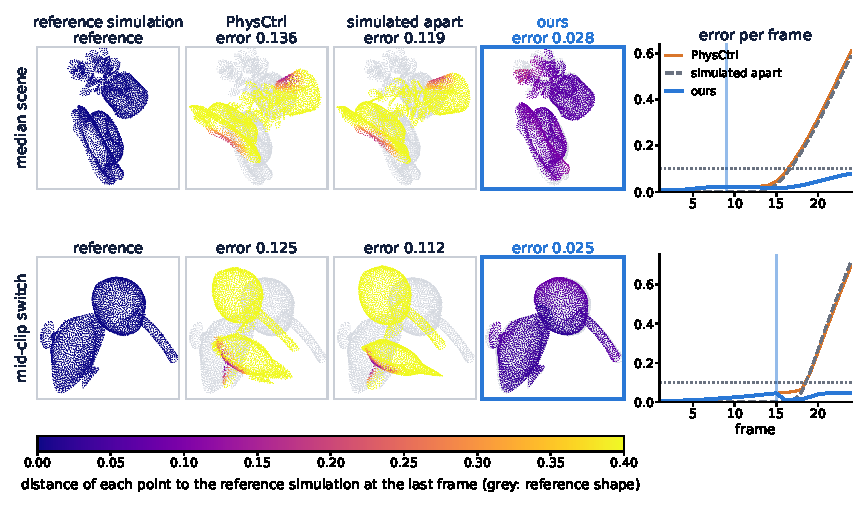
\includegraphics[width=\linewidth]{fig/qual_contact.pdf}
\caption{\textbf{Two-object contact} (fresh test scenes; the median-error scene and the median rejected scene with a mid-clip switch, chosen before any picture). Last frame, side view; colour is each point's distance to the reference. PhysCtrl's composed output nearly coincides with the two objects simulated apart: it ignores the collision. Ours switches to the contact-resolving setting just before contact (blue line).}
\label{fig:qual-contact}
% src: code/fig_paper_select.py, job 94 (recomputed errors match Phase 9 to 4e-7)
\end{figure*}

% ---- moved Oct 21, 2026 (Phase 10c table added to the main paper; page limit) ----
% from sec/5_results.tex, sec:res-cert
\begin{figure}[t]
\centering
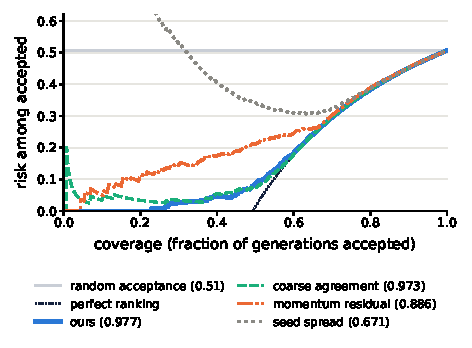
\includegraphics[width=\linewidth]{fig/certificate.pdf}
\caption{\textbf{Ranking generation error} (in-distribution and shifted development queries pooled; AUROC in brackets). Accepting the lowest-scored generations first, the window score stays close to a perfect ranking; PhysCtrl's own uncertainty (seed spread) is worse than random acceptance until most generations are accepted.}
\label{fig:certificate}
% src: results/p7a_metrics (risk_coverage.json, summary.json); code/fig_certificate.py
\end{figure}

% from sec/5_results.tex, sec:res-reference
The tuned settings advance $\lfloor 0.0417/\Delta t\rfloor\Delta t$ seconds per frame, as PhysCtrl's code does, slightly less than the reference's 0.0417\,s; removing this offset lowers their risk under shift by at most 2 points (to at least 8.8\%, 9.3\% and 13.5\%).
% src: PLAN Phase 10 (recorded Oct 20, CPU)

% from sec/5_results.tex, sec:res-negative (main text keeps the first sentence)
Optimising the generation against the window defect lowered the defect while nearly doubling the true error (0.267 to 0.511): the defect is a certificate, not an objective. Certifying the cheap simulator instead of the generator leaked under shift (risk 0.065), and for stiff materials ($E \ge 10^8$\,Pa) the certificate accepted 6 of 16 bad trajectories (both exploratory). An audited amortised verifier skips about 14\% of probes at unchanged risk but saves only 1.3\% (supplement).
% Full Phase 10c table (all pipelines): supp/reference_table_full.tex (code/p10c_table.py)
